Il periodo di Progettazione architetturale ha inizio con la presentazione della RR e finisce con la consegna della RP.\newline
In questo periodo, le attività svolte sono le seguenti:
\begin{itemize}
	\item \textbf{Incremento: }modifiche incrementali ai seguenti documenti, ove necessario:
	\begin{itemize}
		\item Analisi dei requisiti;
		\item Piano di progetto;
		\item Piano di qualifica;
		\item Glossario;
		\item Norme di progetto.
	\end{itemize}
	\item \textbf{Tecnlogy baseline: }decisione delle scelte progettuali ad alto livello.
\end{itemize}

\begin{figure}[H]
	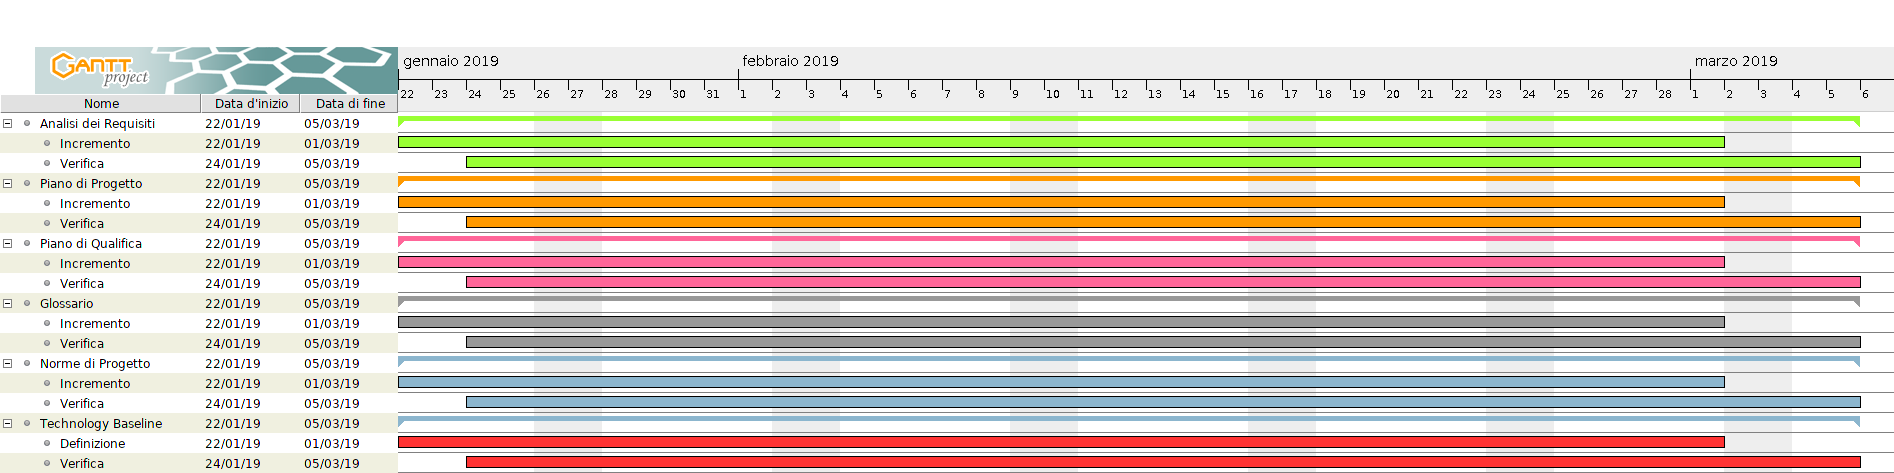
\includegraphics[width=1\linewidth]{Pianificazione/Progettazione_Architetturale_Gantt.png}
	\caption{Diagramma di Gantt del periodo di Progettazione architetturale}
\end{figure}